\documentclass{article}
\usepackage{amsmath}
\usepackage{tikz}
\title{Elements}
\author{DIY.Studying}
\begin{document}
 \maketitle
\section{Basics}
     \begin{itemize}
         \item primitive expressions and statements.
         \item means of combination.
         \item means of abstraction.
     \end{itemize}
\section{expression and statements}
Expression is watch evaluate name to value.And make use of later.If call expression alone and not have side-effect, it can be statements.Statements is a sequences that would excution. And it will change environment of program.
\section{expression}
 \begin{itemize}
     \item expression have value and will band to a name.
     \item expression have evaluate process.
 \end{itemize}
\section{call expression}
 The call expression has subexpressions, which mans of combination.
 \begin{equation*}
     \frac{\operatorname{max}}{\operatorname{oprate}}(\frac{7.5}{\operatorname{operand}},\frac{9.5}{\operatorname{operand}})
 \end{equation*}
  \newpage
 \section{names and environment}
 Name band values.Evaluate name to value,we need consider correlation environment.Name means of abstraction.

 \begin{center}
     \emph{name could band}
 \end{center}
 \begin{enumerate}
     \item improt statements.
     \item assingment operation.
     \item def statements.
 \end{enumerate}
 \section{pure function and non-pure function}
 \emph{Pure functions}. Functions have some input (their arguments) and return some output (the result of applying them).
 \begin{center}
     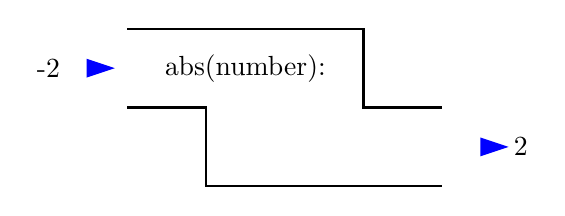
\begin{tikzpicture}
     \node(x) at (3,3.5) {-2};
     \node(y) at (5.5,3.5){abs(number):};
     \draw[thick,blue,fill=blue]
        (3.5,3.6) -- (3.8,3.5) --
        (3.5,3.4) --cycle ;
     \draw[thick]
        (4,4) -- (7,4) --
        (7,3) -- (8,3);
    \draw[thick]
        (4,3) -- (5,3) --
        (5,2) -- (8,2);
    \draw[thick,blue,fill=blue]
        (8.5,2.6) -- (8.8,2.5) --
        (8.5,2.4) --cycle ;
    \node(z) at (9,2.5) {2};
 \end{tikzpicture}
 \end{center}
 \emph{Non-pure functions}. In addition to returning a value, applying a non-pure function can generate side effects, which make some change to the state of the interpreter or computer.
 \begin{center}
     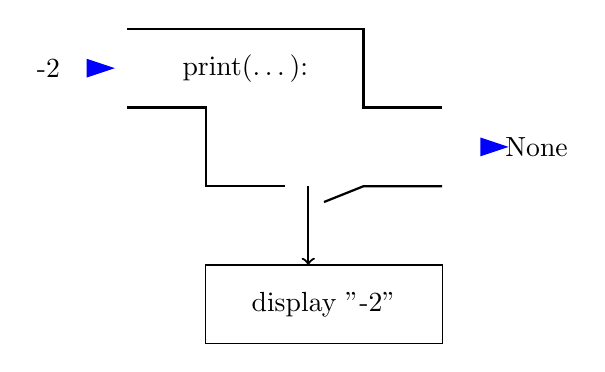
\begin{tikzpicture}
     \node(x) at (3,3.5) {-2};
     \node(y) at (5.5,3.5){print(\ldots):};
     \draw[thick,blue,fill=blue]
        (3.5,3.6) -- (3.8,3.5) --
        (3.5,3.4) --cycle ;
     \draw[thick]
        (4,4) -- (7,4) --
        (7,3) -- (8,3);
    \draw[thick]
        (4,3) -- (5,3) --
        (5,2) -- (6,2);
    \draw[thick]
        (6.5,1.8) -- (7,2) --
        (8,2);
    \draw[thick,blue,fill=blue]
        (8.5,2.6) -- (8.8,2.5) --
        (8.5,2.4) --cycle ;
    \node(z) at (9.2,2.5) {None};
    \draw[->,thick]
        (6.3,2)--(6.3,1);
    \draw (5,0) rectangle (8,1);
    \node(l) at (6.5,0.5){display "-2"};
 \end{tikzpicture}
 \end{center}
\end{document}
